\begin{frame}{Podjęcie akcji}
	
	\begin{columns}
		\begin{column}{.8\hsize}
			\textbf{ruch przód/tył oraz skręt kierownicy}
			\begin{itemize}
				\myitem wartości dyskretne $\{-1, 0, 1\}$
				\myitem wartości ciągłe $[-1, 1]$
			\end{itemize}
			
			\vspace{1cm}
			{\hspace*{7mm}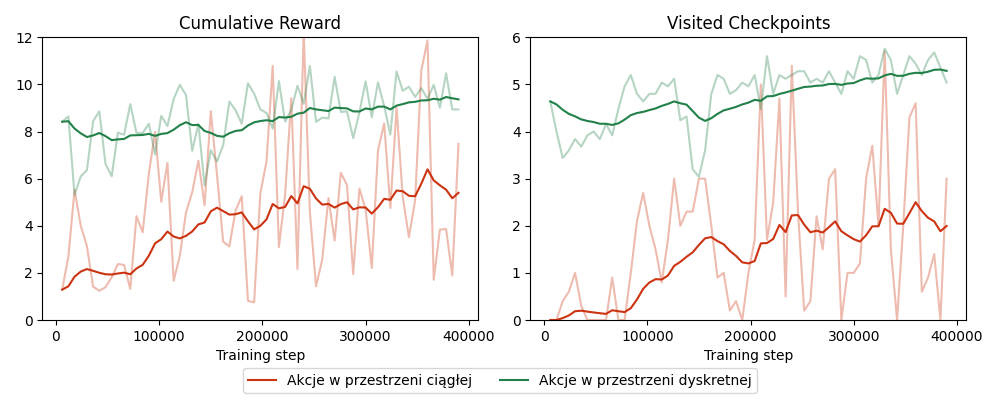
\includegraphics[width=1.2\linewidth]{figures/output_actions.png}}
		\end{column}

		\begin{column}{.2\hsize}
			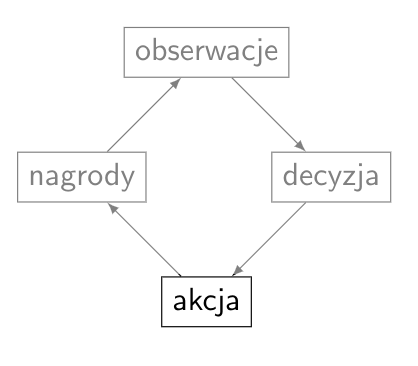
\includegraphics[width=\linewidth]{figures/learning_loop_3.png}
			\vspace{5cm}
		\end{column}
	\end{columns}
	
\end{frame}
